
%%%%%%%%%%%%%%%%%%%%%%%%%%%%%%%%%%%%%
\section{Short term quantum computing}\label{Short term quantum computing}
In this section we aim to give a comprehensive overview of quantum computing platforms which are currently available and discuss the near-term advantages that these platforms can bring.

%%%%%%%%%%%%%%%%%%%%%%%%%%%%%%%%%%%%%%%%%%%%%%%%%%%%%%%%%%%%%%%
\subsection{Adiabatic quantum computing \& quantum annealers}
Dwave, NISC
QUBO problems.

Quantum Algorithms in Dwave? optimisation? Quantum Monte Carlo speed-up? Simulating quantum systems

%%%%%%%%%%%%%%%%%%%%%%%%%%
%%%%%%%%%%%%%%%%%%%%%%%%%%
\subsection{Rigetti- Forest}

%\subsubsection{pyQuil}

Rigetti has created an environment called Forest, amongst its contributions is a python library called PyQuil. With PyQuil one can simulate up to 26 qubits on the Quantum Virtual Machine (QVM). An example code from \cite{rigetti} is detailed below with comments to assist the reader:
\begin{lstlisting}[language=Python]
from pyquil.quil import Program
from pyquil.gates import H, CNOT
from pyquil.api import SyncConnection
# construct a Bell State program
p = Program()
p.inst(H(0))
p.inst(CNOT(0, 1))
# run the program on a QVM
qvm = SyncConnection()
result = qvm.wavefunction(p) 
# produces the output wavefunction of the Bell state
\end{lstlisting}
Rigetti also offers access to a 19 qubit processor they call 19Q. This API 
\begin{lstlisting}[language=Python]
import numpy as np
 
def incmatrix(genl1,genl2):
    m = len(genl1)
    n = len(genl2)
    M = None #to become the incidence matrix
    VT = np.zeros((n*m,1), int)  #dummy variable
 
    #compute the bitwise xor matrix
    M1 = bitxormatrix(genl1)
    M2 = np.triu(bitxormatrix(genl2),1) 
 
    for i in range(m-1):
        for j in range(i+1, m):
            [r,c] = np.where(M2 == M1[i,j])
            for k in range(len(r)):
                VT[(i)*n + r[k]] = 1;
                VT[(i)*n + c[k]] = 1;
                VT[(j)*n + r[k]] = 1;
                VT[(j)*n + c[k]] = 1;
 
                if M is None:
                    M = np.copy(VT)
                else:
                    M = np.concatenate((M, VT), 1)
 
                VT = np.zeros((n*m,1), int)
 
    return M
\end{lstlisting}

\subsubsection{Example Codes}

% \subsubsection{Language} 5

%%%%%%%%%%%%%%%%%%%%%%%%%
%%%%%%%%%%%%%%%%%%%%%%%%%
\subsection{IBM- Project Q}
IBM has launched the IBM Q experience that consists of a development environment called QISkit and a higher-level gate-building platform that allows users to compose their own algorithms. The devices used to perform the simulation and computation are based on a superconducting charge qubit implementation, which can be found described in more detail in \autoref{Implementations}.  This development environment is also based on python, as we saw with Forest by rigetti. There is ample space for development of algorithms in this environment as the visual arrays provide a clear structure to those familiar with quantum computation. The composer also displays the code on which it operates so that users interested in further development have the opportunity to learn how to code their own gates in QISkit. The associated documentation which is linked on the IBM Q website provides more detail to the structure \cite{coles2018quantum}. Updates are regularly posted to the main site. Additional features such as limited access to a larger register of bits are available to academics. Specifications of the device that is being used to perform these calculations are available on the website as seen in \autoref{fig:ibmsite}. 

\begin{figure}[h!]
\centering
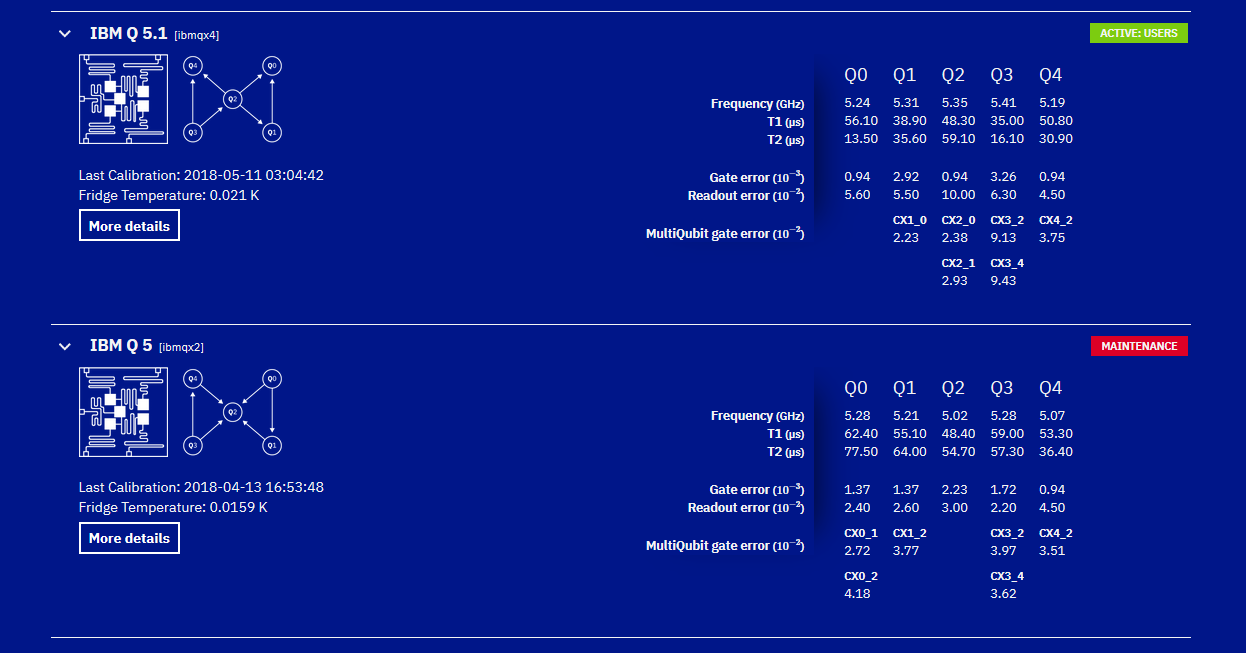
\includegraphics[width=12cm]{ibmsite}
\caption{The description of the devices used for the IBM Q suite as of early May 2018 (must be updated closer to submission). Cooling refrigerator temperature along with the update structure is presented. A useful live display feed allows users to track both the physical and computational side of their own algorithms made on the composer.}
\label{fig:ibmsite}
\end{figure}

\subsubsection{Example Codes}
Examples of composed codes in this environment are based on adding sequences of pre-defined gates. An example of two single-qubit operations being performed on bit 0 out of the 0-4 register.  
\begin{figure}[h!]
\centering
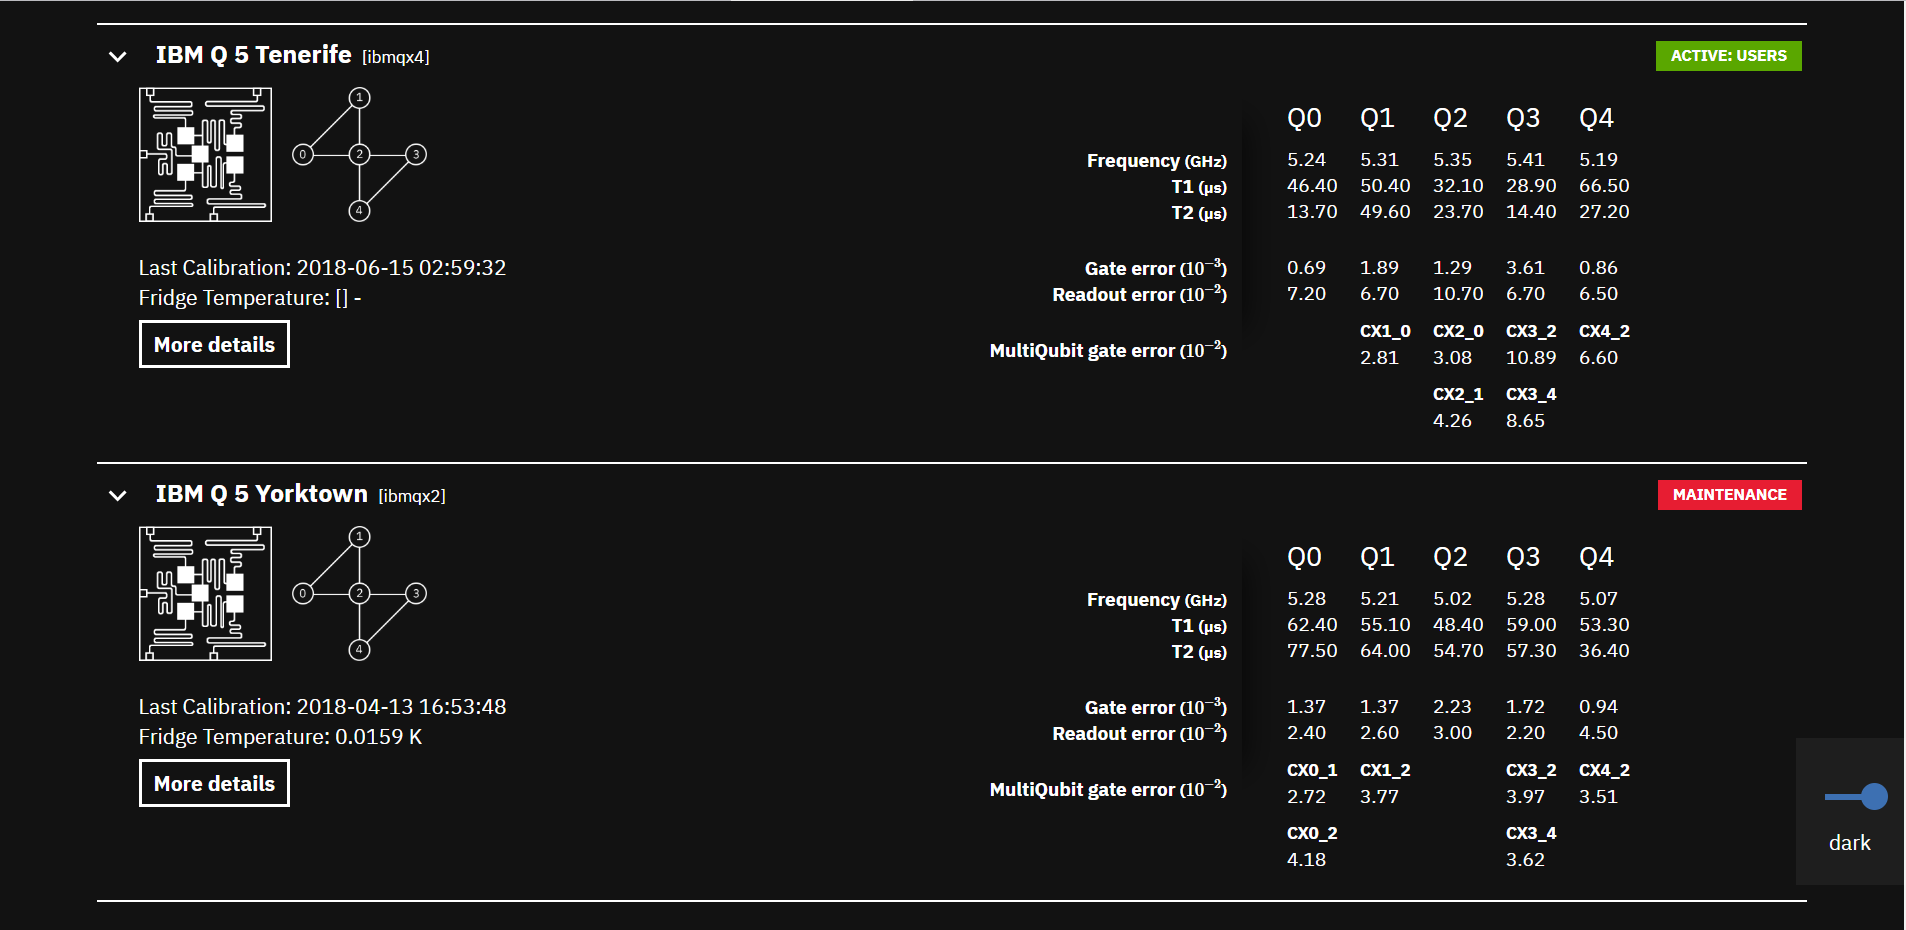
\includegraphics[width=10cm]{IBMq_1}
\caption{An example of the composition suite that allows gates to be strung together. In this instance, the first qubit in the register has the X and Z gates performed on it before measurement. The symbolism is identical to the standard gate model used within this guide, which makes the transition from other environments simpler.}
\end{figure}
%\begin{figure}
%\centering
%\includegraphics[width=10cm]{IBMq_2}
%\caption{In this example, the composition consists of building a set of gates that }
%\end{figure}